\chapter{Introduction}

\section{Objectives and Contributions}
With the overall task being the development of an Android application to monitor skin spots, we can start by breaking the tasks down further, grouping the three core goals into Technical, Evaluation and Publishing tasks.
\begin{enumerate}
    \item \textbf{Technical Tasks:}
    \begin{enumerate}
        \item The user can add and name new spots, additionally, the user can add new images to a spot.
        \item The user is able to compare two images of a spot on the same screen.
        \item The ability to email both pictures to a doctor from within the app.
        \item Educational information screens towards skin cancer signs and usage of the app.
    \end{enumerate}
    \item \textbf{Evaluation Tasks:}
    \begin{enumerate}
        \item Performing Alpha and Beta testing phases for bug fixing and app improvements.
        \item Carry out a usability analysis with known human factor assessment methodologies.
    \end{enumerate}
    \item \textbf{Publishing Tasks:}
    \begin{enumerate}
        \item Reworking of the TrackYourSpot website to accommodate for both the iOS and Android versions of the app.
        \item Publishing a stable version of the app on the Android Play Store.
    \end{enumerate}
\end{enumerate}

\section{Definition of Terms}
Some of the language used in this report can appear confusing for people unfamiliar with the Android platform. These terms are used continually throughout the report so it is recommended to pay close attention to the following definitions:
\begin{itemize}
    \item \textbf{Google Play Store} - The Android application store/market, users can choose from over 2.5 million apps to download \cite{appbrain_2019}.
    \item \textbf{Activity} - An application component, displayed as a single screen to the user. Each screen has its own activity. Activities contain the code that interacts with the UI.
    \item \textbf{Fragment} - Similar to an activity, but a fragment only occupies part of the screen. Multiple fragments can be used in a screen, and fragments can be swapped within an activity.
    \item \textbf{XML Layout} - Each Activity has its own XML file controlling the visual appearance of the screen. The code inside the activity can interact with elements described in the XML file.
    \item \textbf{Android API} - In an Android context, it refers to the version number of the operating system. For example, API 23 stands for the \emph{Marshmallow} Android version.
    \item \textbf{SDK} - Formally refers to a Software Development Kit, however, in the Android context, it is also used to refer to the Android version. For example, the \emph{minimumSDK} of an app is the minimum Android version required to run the app.
    \item \textbf{Intent} - A messaging object to request an action from another app component. Intents are used to change from one activity to another, among others.
    \item \textbf{APK} - The package file format used to distribute and install an app. This file can be uploaded to the Google Play Store.
\end{itemize}
For full definitions and examples, please refer to the Android docs \cite{androidfullguide}.

Throughout the report, Activities will occasionally be referred to by their implementation class name, for example, \emph{CompareScreen} refers to the spot comparison screen, while \emph{SpotImageList} refers to the screen displaying all the images of a same spot.

\section{Related Work}
This section will evaluate similar android apps in the Google Play Store, finding possible flaws with them and justifying the gap in the market for our application. After scouting the Google Play Store, three main apps seem to be dominating the skin spot tracking market. As labelled on the app store, they are:
\begin{itemize}
    \item Miiskin - Melanoma Skin Cancer
    \item Molexplore "Skin Cancer App"
    \item SkinVision - Detect Skin Cancer
\end{itemize}
Each subsection below will analyse them individually, evaluating the respective advantages and disadvantages of each by testing out the different apps.
\subsection{Miiskin - Melanoma Skin Cancer}
With over 100,000 downloads and 1000+ reviews, it is no surprise that this app appears as the first result when searching for "Skin Cancer" in the Google Play Store. The app averages 4.2/5 stars and has a premium subscription of \pounds2.99 a month or \pounds23.49 a year. Figure \ref{fig:miiskin} shows a screenshot of the app listing on the Google Play Store. The app allows taking photos of moles, setting up reminders to update a mole, and comparing two photos of a mole side by side.
\begin{figure}
    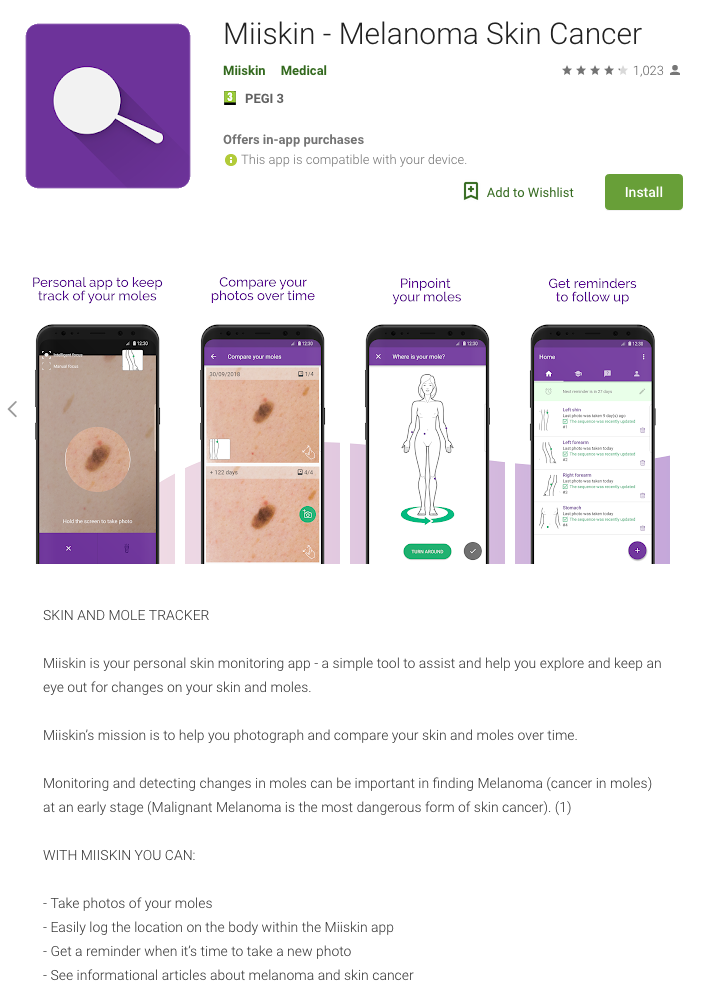
\includegraphics[width=1\textwidth, center]{figures/miiskin_listing.png}
    \caption{MiiSkin Google Play Store's Listing}
    \label{fig:miiskin}
\end{figure}

Advantages:
\begin{itemize}
    \item The user can pinpoint the exact location of body spots, this helps with identifying different spots in the same body part. Sometimes spots can look very similar, if the user adds a photo to the wrong spot, it would hinder the comparison task. This model prevents this from happening.
    \item Ability to zoom into pictures while comparing them. This addresses the issue of users cropping images to incorrect sizes, as they can just zoom in on this screen instead.
    \item Reminders to take photos of a spot through push notifications. This is a particularly useful feature, as it could make the difference between one-time app users and regular users, updating their spots once every few weeks.
\end{itemize}

Disadvantages:
\begin{itemize}
    \item While marketed as a free app, the app is only usable through a trial version, requiring payment details before registering. The user's photos become inaccessible once the free trial version runs out, frustrating many of its users.
    \item Users are forced to register if they want to use the app, this can put many people off who just want to quickly try out the app, as they might only be interested in the offline features of the app.
\end{itemize}

\subsection{Molexplore "Skin Cancer App"}
Second in the list, one can find this skin spot tracking app. The app has 50,000 downloads and 347 reviews (Figure \ref{fig:molexplore}), averaging 4/5 stars. The app offers similar core features as MiiSkin, it allows pinpointing the exact location of spots, comparing images side by side and offering general skin health information. The app is completely free to use.
\begin{figure}
    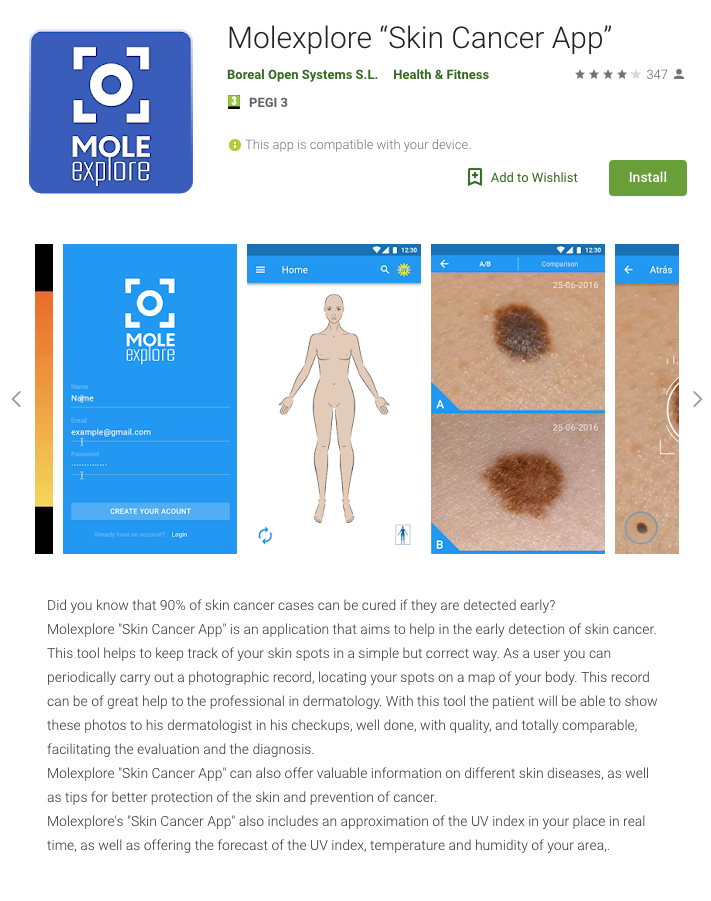
\includegraphics[width=1\textwidth, center]{figures/molexplore_listing.png}
    \caption{Molexplore Google Play Store's Listing}
    \label{fig:molexplore}
\end{figure}

Advantages:
\begin{itemize}
    \item The app provides very helpful insight on what to look for when inspecting skin spots, for example, it offers advice on interpreting the color, symmetry, borders or diameter of a spot.
    \item An alternative way of comparing spots is available, it's called "Overlap Compare". This feature blends both images together to a user specified degree. This feature would be particularly useful in detecting changes in size or shape of a spot.
    \item The app provides real time UV radiation index information custom to the user's location. While it isn't essential for the process of adding and comparing images, it could be useful information for the user.
\end{itemize}

Disadvantages:
\begin{itemize}
    \item The app's UI can seem a bit clunky or "old". Adding or comparing spots seems to require more steps than the two previous applications.
    \item Even if the app doesn't offer any online features, it also requires registration before use. This is once again a drawback for some users.
    \item Recent user reviews have complained about frequent crashes in different areas of the app. This is an indicator of a buggy implementation or a lack of maintenance from the Molexplore team.
\end{itemize}

\subsection{SkinVision - Detect Skin Cancer}
This app also surpasses 100,000 downloads. It averages 3/5 stars with 883 reviews (Figure \ref{fig:skinvision}). Contrarily to the previous two apps, this app provides a slightly different service. The app offers a "clinically validated algorithm" that actually detects instances of skin cancer. The app's business model is also quite unique. It offers one free "Smart Check", giving the user a risk indication on a photo of a skin spot, risky spots are also inspected by their team of dermatologists to provide further advice. After this free trial, users can choose to pay \pounds3.99 for one individual "Smart Check" or pay \pounds21.99 a year for an unlimited amount.
\begin{figure}
    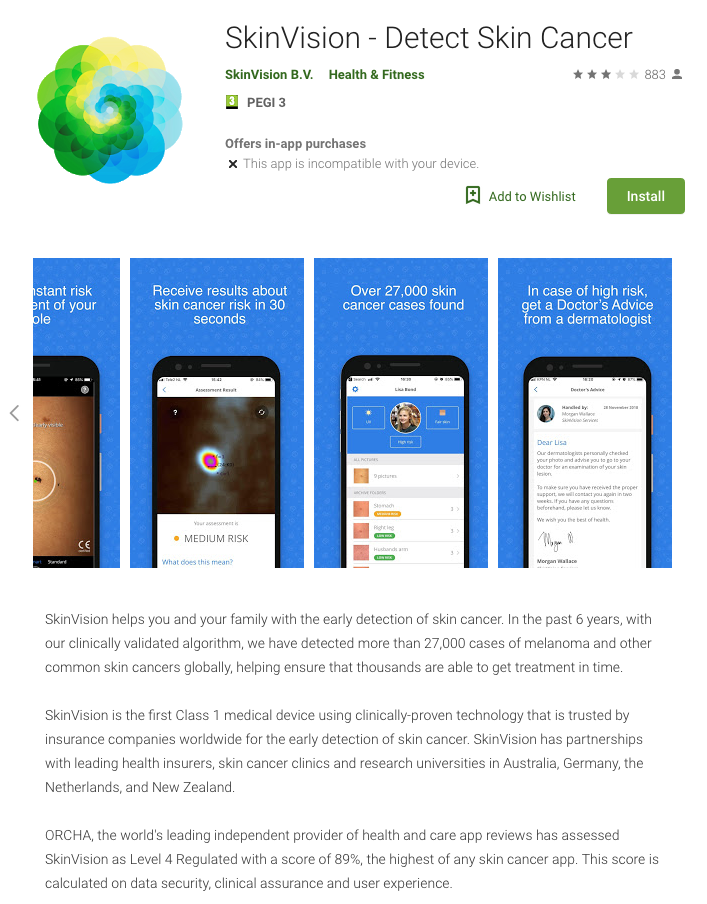
\includegraphics[width=1\textwidth, center]{figures/skinvision_listing.png}
    \caption{SkinVision Google Play Store's Listing}
    \label{fig:skinvision}
\end{figure}

Advantages:
\begin{itemize}
    \item The app provides an actual diagnosis with a spot risk assessment and doctor attention if required. This is an incredibly valuable feature which will be realistically impossible to compete with.
    \item Email, SMS and push notification reminders are available for any previously added spot, this goes the extra mile in preventing the user from just "swiping away" a notification.
\end{itemize}

Disadvantages:
\begin{itemize}
    \item The obvious main issue of this app is the price. A payment of \pounds3.99 for a single check is a very expensive price to pay for tracking a spot. Given the service they claim to offer, it is clear the app is targeted more towards people seeking for medical attention or heavily worried about particular skin lesions. 
\end{itemize}

\subsection{Conclusion}
It would be unreasonable to aim for an app of SkinVision's characteristics, as the both the legal implications and scope would be unrealistic for an undergraduate project such as this one. Additionally, given that our target user is more of a casual user looking to monitor his skin spots, it would be sensible to assume SkinVision in a different category. Furthermore, even if all three apps are developed and maintained by a team of developers, comparing our app to Miiskin and Molexplore would be more logical.

From the evaluations of both apps, the following five points will prove to be decisive if the app aims to compete in the skin spot tracking app market:
\begin{enumerate}
    \item \textbf{Free Business Model} - The app will offer users a completely free way of monitoring their skin spots, no ads or in-app purchases will be offered. This business model will be exactly the same as Molexplore's, so the app's success will depend on the other features.
    \item \textbf{Good Information Screens} - The app will have to offer relevant and insightful information screens about skin spot tracking.
    \item \textbf{Intuitive UI} - The app's UI will have to be easy to use and intuitive. Making the app easy to understand is the first step to attract new users.
    \item \textbf{Email Functionaility} - The email functionality is not offered by any of the other apps. This feature could somewhat emulate SkinVision's medical attention feature, even if user's would have to input their own doctor's email address.
    \item \textbf{App Stability} - Needless to say, the app being bugfree and compatible with as many devices as possible will be very important in ensuring users don't delete the app.
\end{enumerate}

\section{Report Structure}
The content of this report will be the following:
\begin{itemize}
    \item \textbf{Chapter 2 - Design: } A collection of User Interface app designs, justification for design decisions of the main screens and specific UI features, as well as interactions used within the app.
    \item \textbf{Chapter 3 - Architecture and Implementation: }This chapter will delve into the technical challenges of the task. Including choices for object architecture, alternative and/or unsuccessful approaches, flow of data and core algorithms.
    \item \textbf{Chapter 4 - Deployment: }Everything involved with publishing and branding of the app. It also contains a section dedicated to the TrackYourSpot website.
    \item \textbf{Chapter 5 - User Testing and Evaluation: } Code Testing phases and exploring the human factor element of the project. Analysis and results of usability testing methods and evaluation of these are also included.
    \item \textbf{Chapter 6 - Conclusion: }Overall result of the project, limitations, lessons learnt and future work.
\end{itemize}